% Reviewed translation: PDF pages 173--179 / printed pages 159--165.
% Continues the proof opened in chapter-02-section-03-part-01.tex.
\MathBookSourcePage{173}

考虑一个由仿射映射 $F$ 与 $\kappa$ 联系的``参考''集合 $\hat\kappa$,
它未必是单位正方形. 更准确地说, 将 $\kappa$ 分为两个子三角形(见
Figure~\ref{fig:primitive-quadrilateral-affine-subtriangles}):
\[
\kappa=S_1\cup S_3.
\]
设 $\hat S_1$ 为参考单位三角形, $F$ 为满足
\[
S_1=F(\hat S_1),
\qquad F(\hat x)=B\hat x+b
\]
的仿射映射, 并令
\[
\hat S_3=F^{-1}(S_3).
\]
换言之,
\[
\hat\kappa=\hat S_1\cup\hat S_3,
\qquad\kappa=F(\hat\kappa).
\]
由于 $F$ 为仿射映射且 $\kappa$ 为凸集, 参考集合 $\hat\kappa$ 也是凸四边形.
此外, 一方面立即得到
\[
\operatorname{meas}(\hat S_i)
=\frac12\frac{\operatorname{meas}(S_i)}{\operatorname{meas}(S_1)},
\qquad1\leq i\leq4,
\]
其中 $\hat S_i$(相应地 $S_i$)表示 $\hat\kappa$(相应地 $\kappa$)的四个子三角形之一.
另一方面, $\hat\kappa$ 的任意两个顶点满足
\[
\hat a_i-\hat a_j=B^{-1}(a_i-a_j).
\]
此外, \eqref{eq:appendix-simplex-matrix-bounds} 在这里给出
\[
\|B\|\leq\frac32h_{S_1},
\qquad\|B^{-1}\|\leq\frac{\sqrt2}{\rho_{S_1}},
\qquad|\det(B)|=2\operatorname{meas}(S_1).
\]

现在取 $f\in H^k(\kappa)$, $0\leq k\leq l$. $P_{l-1}$ 上的
$L^2$ 投影 $\rho_h$ 在仿射变换下不变. 因而
\[
\|f-\rho_hf\|_{0,\kappa}
=|\det(B)|^{1/2}\|\hat f-\hat\rho\hat f\|_{0,\hat\kappa}.
\]
但对 $0\leq j\leq l-1$,
\[
\|\hat f-\hat\rho\hat f\|_{0,\hat\kappa}
\leq\inf_{q\in P_j}\|\hat f+q\|_{0,\hat\kappa}
=\|\hat f\|_{L^2(\hat\kappa)/P_j}.
\]
由于 $\hat\kappa$ 是可变四边形, 必须明确满足
\[
\|\hat f\|_{L^2(\hat\kappa)/P_j}
\leq C(\hat\kappa)|\hat f|_{j+1,\hat\kappa}
\]
的常数 $C(\hat\kappa)$. 对次数 $j$ 作归纳. 当 $j=0$ 时, 这是唯一可用
Theorem~\ref{thm:appendix-quadrilateral-bramble-hilbert} 的情形, 得
\[
\|\hat f\|_{L^2(\hat\kappa)/P_0}
\leq C_1h_{\hat\kappa}
\left[\frac{\max_i\operatorname{meas}(\hat S_i)}
{\min_i\operatorname{meas}(\hat S_i)}\right]^{1/2}
|\hat f|_{1,\hat\kappa},
\]
其中 $C_1$ 与 $h,\hat\kappa,f$ 无关. 关于 $\hat\kappa$ 几何性质的上述观察表明
\[
\left[\frac{\max_i\operatorname{meas}(\hat S_i)}
{\min_i\operatorname{meas}(\hat S_i)}\right]^{1/2}
\leq C_2\sigma_\kappa,
\qquad h_{\hat\kappa}\leq C_3\sigma_\kappa.
\]

\MathBookSourcePage{174}
因此
\begin{equation}\label{eq:primitive-quadrilateral-projection-induction-base}
\|\hat f\|_{L^2(\hat\kappa)/P_0}
\leq C_4\sigma_\kappa^2|\hat f|_{1,\hat\kappa}.
\end{equation}
接着假设
\begin{equation}\label{eq:primitive-quadrilateral-projection-induction}
\|\hat f\|_{L^2(\hat\kappa)/P_{j-1}}
\leq(C_4\sigma_\kappa^2)^j|\hat f|_{j,\hat\kappa}.
\end{equation}
可写成
\[
\begin{aligned}
\|\hat f\|_{L^2(\hat\kappa)/P_j}
&=\inf_{(q,\tilde q)\in P_{j-1}\times\widetilde P_j}
\|\hat f+q+\tilde q\|_{0,\hat\kappa}\\
&=\inf_{\tilde q\in\widetilde P_j}\inf_{q\in P_{j-1}}
\|\hat f+\tilde q+q\|_{0,\hat\kappa}\\
&\leq(C_4\sigma_\kappa^2)^j
\inf_{\tilde q\in\widetilde P_j}|\hat f+\tilde q|_{j,\hat\kappa},
\end{aligned}
\]
其中使用了归纳假设 \eqref{eq:primitive-quadrilateral-projection-induction}.
再由 \eqref{eq:primitive-quadrilateral-projection-induction-base} 得
\[
\|\hat f\|_{L^2(\hat\kappa)/P_j}
\leq(C_4\sigma_\kappa^2)^{j+1}
\left\{\sum_{|\alpha|=j}|\partial^\alpha\hat f|_{1,\hat\kappa}^2\right\}^{1/2}.
\]
花括号中的表达式就是 $|\hat f|_{j+1,\hat\kappa}$, 因而对所有 $j$
证明了 \eqref{eq:primitive-quadrilateral-projection-induction}. 于是
\[
\|f-\rho_hf\|_{0,\kappa}
\leq(C_4\sigma_\kappa^2)^k|\det(B)|^{1/2}|\hat f|_{k,\hat\kappa},
\]
而 \eqref{eq:appendix-change-forward} 和 $\mathcal T_h$ 的正则性给出
\eqref{eq:primitive-quadrilateral-pressure-projection}.
\end{Proof}

由 Lemma~\ref{lem:primitive-quadrilateral-pressure-projection},
\eqref{eq:primitive-quadrilateral-higher-velocity-interpolation} 和
Theorem~\ref{thm:primitive-quadrilateral-local-inf-sup}, 得到该格式的预期估计.

\setcounter{statement}{2}
\renewcommand{\theHstatement}{theorem.\thesection.\arabic{statement}}
\begin{Theorem}\label{thm:primitive-quadrilateral-higher-convergence}
设 $\Omega$ 为有界平面多边形, 并假设 Stokes 系统的解 $(\mathbf u,p)$ 满足
\[
\mathbf u\in[H^{k+1}(\Omega)\cap H_0^1(\Omega)]^2,
\qquad p\in H^k(\Omega)\cap L_0^2(\Omega),
\]
其中某个整数 $k\in[1,l]$. 若三角剖分 $\mathcal T_h$ 正则, 则采用
\eqref{eq:primitive-quadrilateral-higher-velocity-spaces} 和
\eqref{eq:primitive-quadrilateral-higher-pressure-spaces} 定义的空间 $X_h,M_h$ 时,
\eqref{eq:primitive-discrete-q-first}--\eqref{eq:primitive-discrete-p}
的解 $(\mathbf u_h,p_h)$ 满足
\[
\|\mathbf u-\mathbf u_h\|_{1,\Omega}+\|p-p_h\|_{0,\Omega}
\leq C_1h^k\{\|\mathbf u\|_{k+1,\Omega}+|p|_{k,\Omega}\}.
\]
此外, 若 $\Omega$ 为凸集, 则有 $L^2$ 估计
\[
\|\mathbf u-\mathbf u_h\|_{0,\Omega}
\leq C_2h^{k+1}(\|\mathbf u\|_{k+1,\Omega}+|p|_{k,\Omega}).
\]
\end{Theorem}

\subsection{棋盘格不稳定性的例子: $Q_1$--$P_0$ 单元}
\label{subsec:primitive-q1-p0-element}

不满足 inf-sup 条件的空间中最著名的例子是: 在矩形网格上, 速度由分片
$Q_1^2$ 多项式组成, 压力为分片常数. 这一组合通常称为 ``$Q_1$--$P_0$'' 单元.

\MathBookSourcePage{175}
更准确地说, 假设 $\Omega$ 是各边平行于坐标轴的有界多边形, 并为简化起见假设
$\mathcal T_h$ 为正方形网格. 取
\begin{equation}\label{eq:primitive-q1-p0-spaces}
\left\{
\begin{aligned}
X_h&=\{\,\mathbf v_h\in\mathcal C^0(\bar\Omega)^2;
\ \mathbf v_h|_\kappa\in Q_1^2\quad\forall\kappa\in\mathcal T_h,
\ \mathbf v_h|_\Gamma=0\,\},\\
M_h&=\{\,q_h\in L_0^2(\Omega);
\ q_h|_\kappa\in P_0\quad\forall\kappa\in\mathcal T_h\,\}.
\end{aligned}
\right.
\end{equation}

\begin{figure}[htbp]
\centering
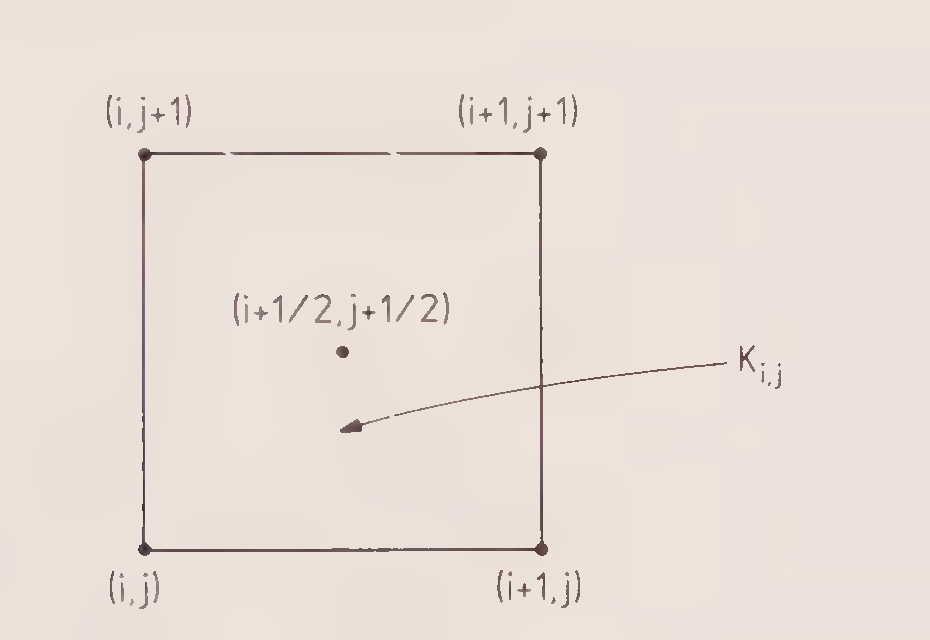
\includegraphics[width=.42\linewidth]{figures/chapter-02-figure-12.png}
\caption{正方形单元 $\kappa_{i,j}$ 及其节点编号.}
\label{fig:primitive-square-cell-indexing}
\end{figure}

这对空间很早以前便已提出; 由于它非常简单, 许多数值分析工作者和工程师曾经并且
仍在使用它处理 Stokes 问题. 然而, 近似压力中的数值不稳定性很快表明,
这种空间选择存在问题.

\eqref{eq:primitive-q1-p0-spaces} 最明显的异常是
$\operatorname{Ker}(B_h')$ 并不退化为 $\{0\}$. 事实上, 如
Figure~\ref{fig:primitive-square-cell-indexing} 那样用 $(i,j)$ 对 $\mathcal T_h$
的节点作 Cartesian 编号; 令 $\kappa_{i,j}$ 表示左下顶点为 $(i,j)$ 的正方形,
令 $(i+1/2,j+1/2)$ 表示 $\kappa_{i,j}$ 中心的指标. 为简化记号, 以
$\mathbf v=(u,v)$ 表示 $X_h$ 中的函数, 以 $u_{i,j}$ 或 $v_{i,j}$ 表示 $u$
或 $v$ 在节点 $(i,j)$ 处的值; 类似地, 以 $q_{i+1/2,j+1/2}$ 表示 $q$
在 $\kappa_{i,j}$ 中心的值. 因为 $q\in M_h$ 在 $\kappa_{i,j}$ 上为常数,
立即得到
\[
\begin{aligned}
\int_{\kappa_{i,j}}q\operatorname{div}\mathbf v\,dx
&=h^2q_{i+1/2,j+1/2}(\operatorname{div}\mathbf v)_{i+1/2,j+1/2}\\
&=h^2q_{i+1/2,j+1/2}\frac1{2h}
\{(u_{i+1,j+1}+u_{i+1,j}-u_{i,j+1}-u_{i,j})\\
&\hspace{42mm}+(v_{i+1,j+1}+v_{i,j+1}-v_{i+1,j}-v_{i,j})\}.
\end{aligned}
\]
于是分部求和给出
\begin{equation}\label{eq:primitive-q1-p0-summation-by-parts}
\int_\Omega q\operatorname{div}\mathbf v\,dx
=-h^2\sum_{i,j}\{u_{i,j}(\nabla_1q)_{i,j}
+v_{i,j}(\nabla_2q)_{i,j}\},
\end{equation}
其中

\MathBookSourcePage{176}
\begin{equation}\label{eq:primitive-q1-p0-discrete-gradients}
\left\{
\begin{aligned}
(\nabla_1q)_{i,j}
&=\frac1{2h}(q_{i+1/2,j+1/2}+q_{i+1/2,j-1/2}
-q_{i-1/2,j+1/2}-q_{i-1/2,j-1/2}),\\
(\nabla_2q)_{i,j}
&=\frac1{2h}(q_{i+1/2,j+1/2}+q_{i-1/2,j+1/2}
-q_{i+1/2,j-1/2}-q_{i-1/2,j-1/2}).
\end{aligned}
\right.
\end{equation}
求和遍历 $\mathcal T_h$ 的所有内部节点 $(i,j)$, 因为 $\mathbf v$ 在 $\Gamma$ 上为零.
因此, 若 $q\in\operatorname{Ker}(B_h')$, 即 $q\in M_h$ 且
\[
\int_\Omega q\operatorname{div}\mathbf v\,dx=0
\qquad\forall\mathbf v\in X_h,
\]
则必有
\[
q_{i+1/2,j+1/2}=q_{i-1/2,j-1/2},
\qquad
q_{i-1/2,j+1/2}=q_{i+1/2,j-1/2}.
\]

\begin{figure}[htbp]
\centering
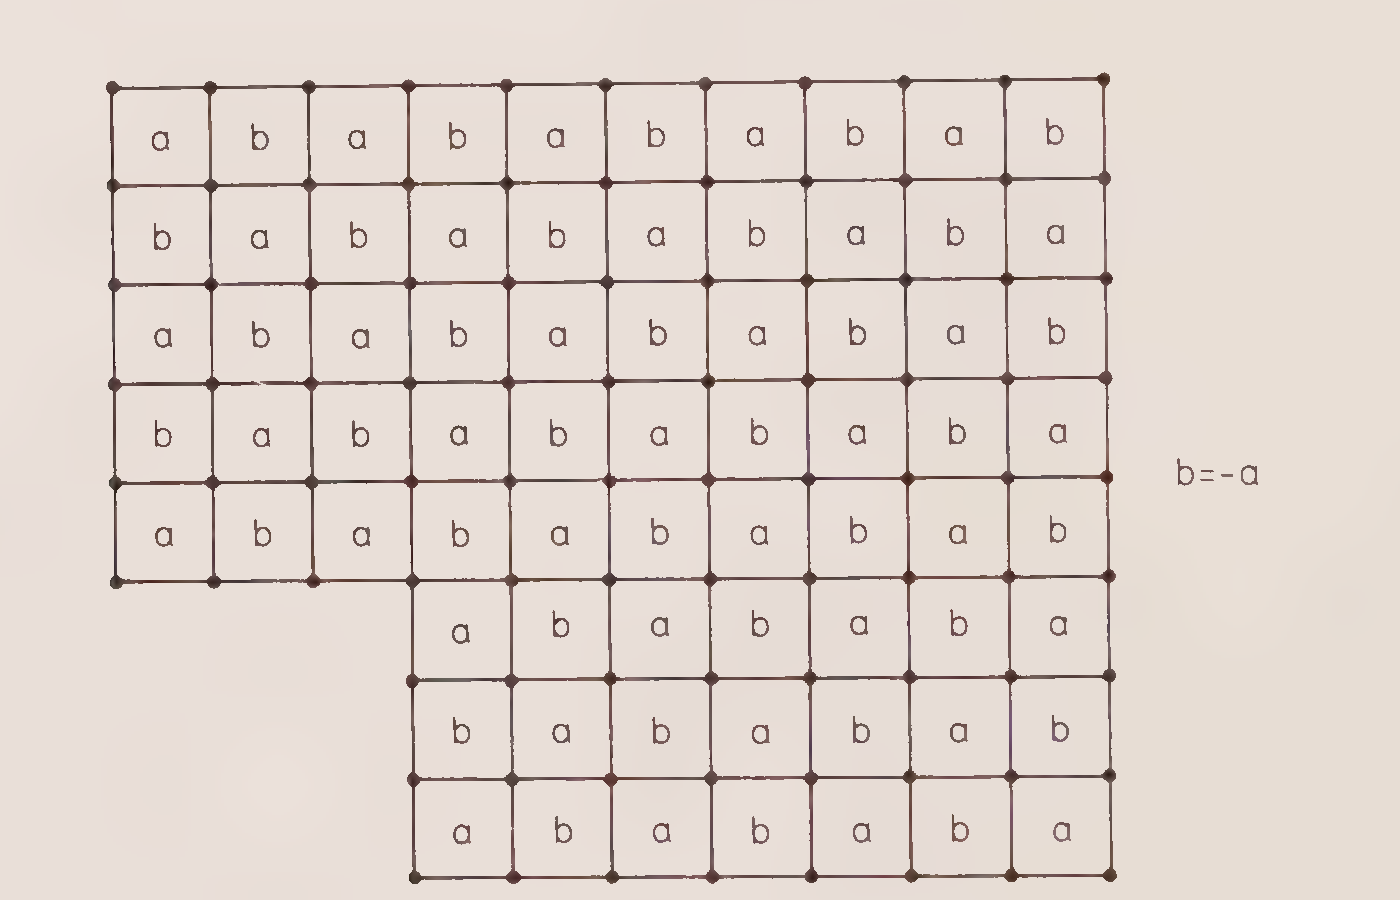
\includegraphics[width=.62\linewidth]{figures/chapter-02-figure-13.png}
\caption{相邻单元上的交替压力值.}
\label{fig:primitive-checkerboard-pattern}
\end{figure}

这些等式未必意味着 $q$ 在 $\Omega$ 中为常数. 相反, 如
Figure~\ref{fig:primitive-checkerboard-pattern} 所示, $q$ 的值可以在相邻单元上
于两个常数之间交替. 由 $\int_\Omega q\,dx=0$ 可知这两个常数必须互为相反数.

下面更精确地刻画 $\operatorname{Ker}(B_h')$. 为简化讨论, 设
$\Omega=(-1,1)\times(-1,1)$, 且 $\mathcal T_h$ 是网格尺寸
\[
h=1/(2n)
\]
的偶数正方形网格, 其节点为
\[
x_{i,j}=(ih,jh),
\qquad-2n\leq i,j\leq2n
\]
(见 Figure~\ref{fig:primitive-even-square-grid}). 定义 $\mu\in M_h$:
\begin{equation}\label{eq:primitive-checkerboard-function}
\mu|_{\kappa_{i,j}}=(-1)^{i+j}
\qquad\forall\kappa_{i,j}\subset\mathcal T_h.
\end{equation}

\MathBookSourcePage{177}
\begin{figure}[htbp]
\centering
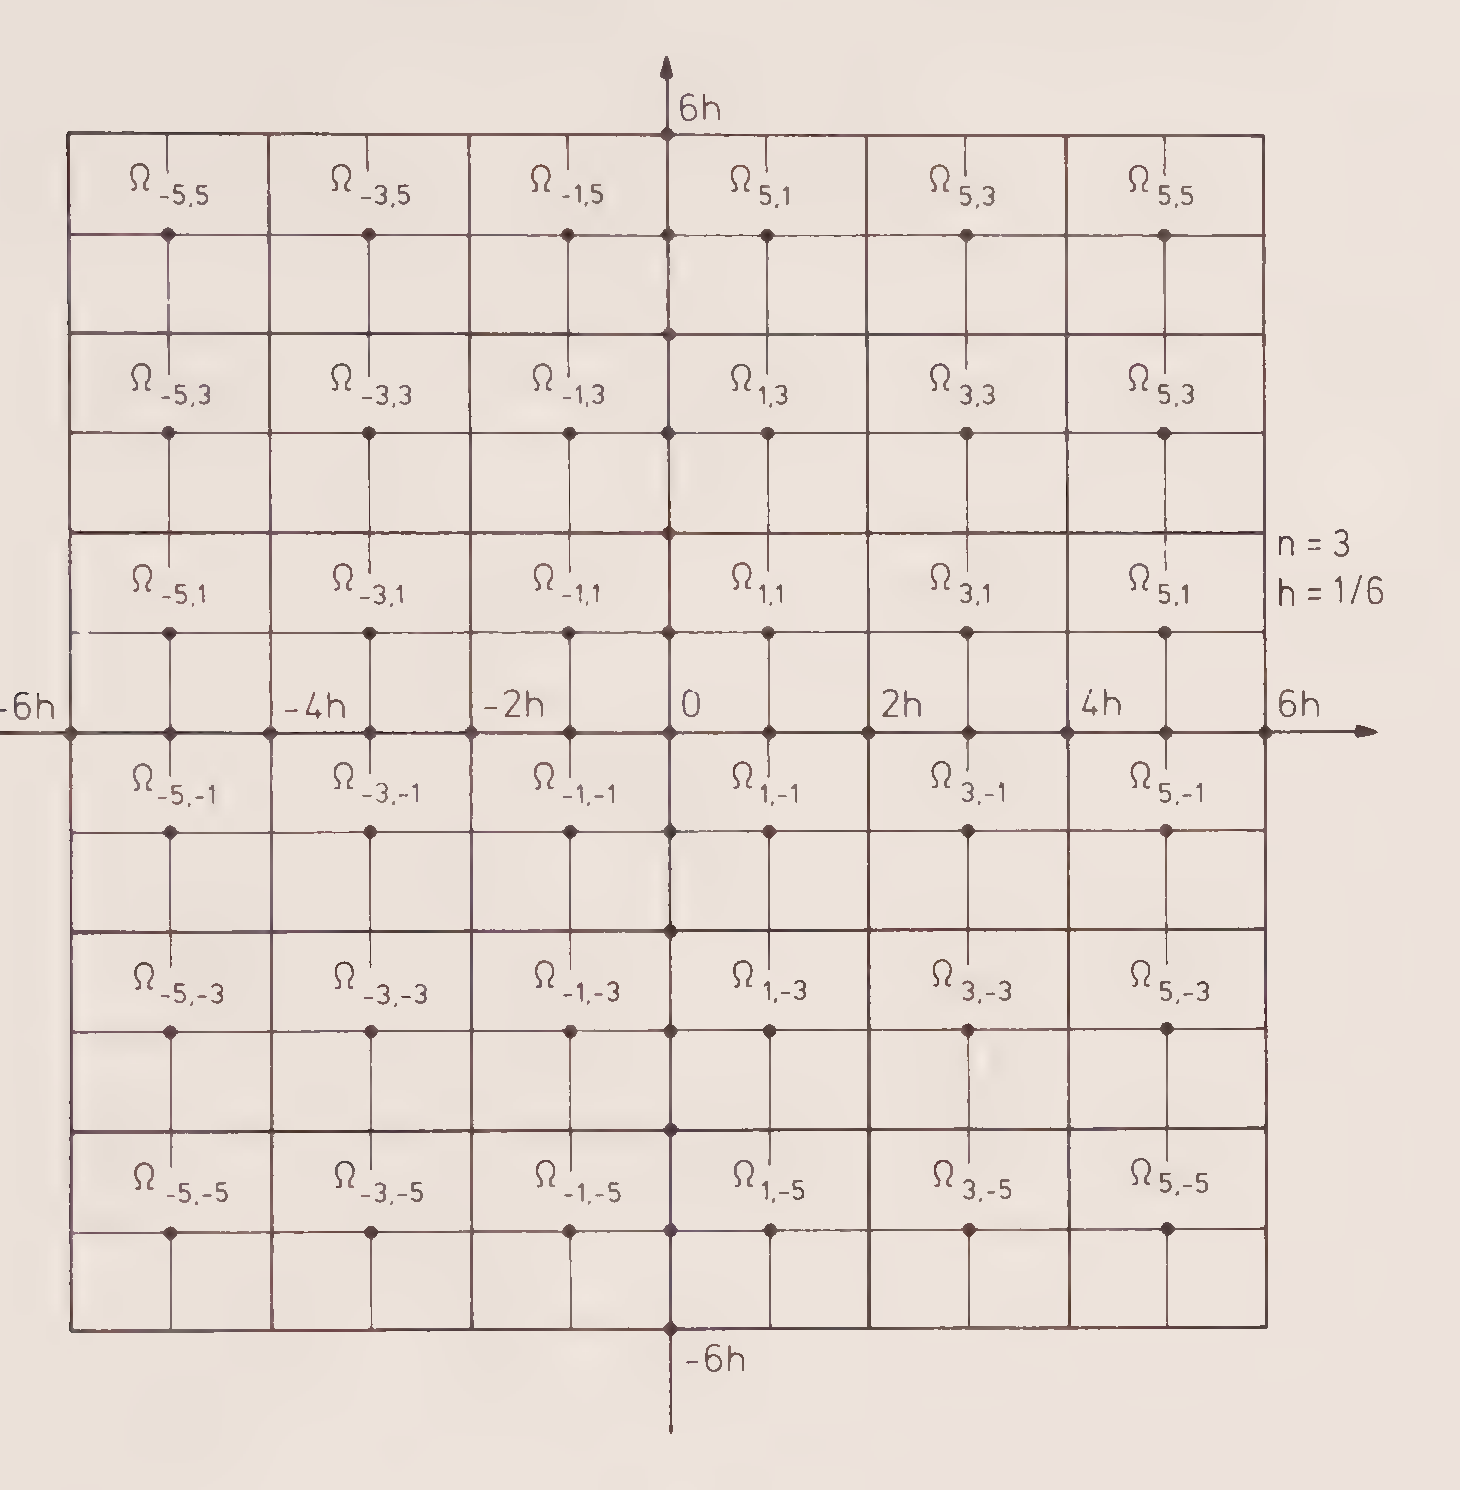
\includegraphics[width=.62\linewidth]{figures/chapter-02-figure-14.png}
\caption{偶数正方形网格及其宏单元.}
\label{fig:primitive-even-square-grid}
\end{figure}

由上述讨论得
\begin{equation}\label{eq:primitive-q1-p0-kernel}
\operatorname{Ker}(B_h')=\operatorname{span}(\mu).
\end{equation}
由于 $\mu$ 具有交替的``正负''图案, 它称为棋盘格函数. Fortin [28]
最先报道了它与 $\operatorname{Ker}(B_h')$ 的联系, 随后 Sani et al. [70]
也作了报道.

由 \eqref{eq:primitive-q1-p0-kernel}, 空间对 $(X_h,M_h)$ 不可能满足 inf-sup 条件.
为补救这一问题, 第一步可以把 $M_h$ 替换为 $[\operatorname{Ker}(B_h')]^\perp$.
下面刻画此空间. 对 $-n\leq i,j\leq n-1$, 令 $I=2i+1,J=2j+1$,
并令宏单元 $\Omega_{I,J}$ 为共享顶点 $(I,J)$ 的四个正方形 $\kappa$ 之并.
按照 Johnson \& Pitkäranta [46], 对每个 $(I,J)$ 引入四个函数
$(v_k)_{I,J}$, $1\leq k\leq4$, 它们依照
Figure~\ref{fig:primitive-macroelement-basis} 的图案在 $\Omega_{I,J}$
的子正方形上取值 $\pm1$. 注意
\begin{equation}\label{eq:primitive-macroelement-basis-means}
\int_{\Omega_{I,J}}(v_k)_{I,J}\,dx=0
\qquad\text{当 }k\neq1.
\end{equation}

\MathBookSourcePage{178}
\begin{figure}[htbp]
\centering
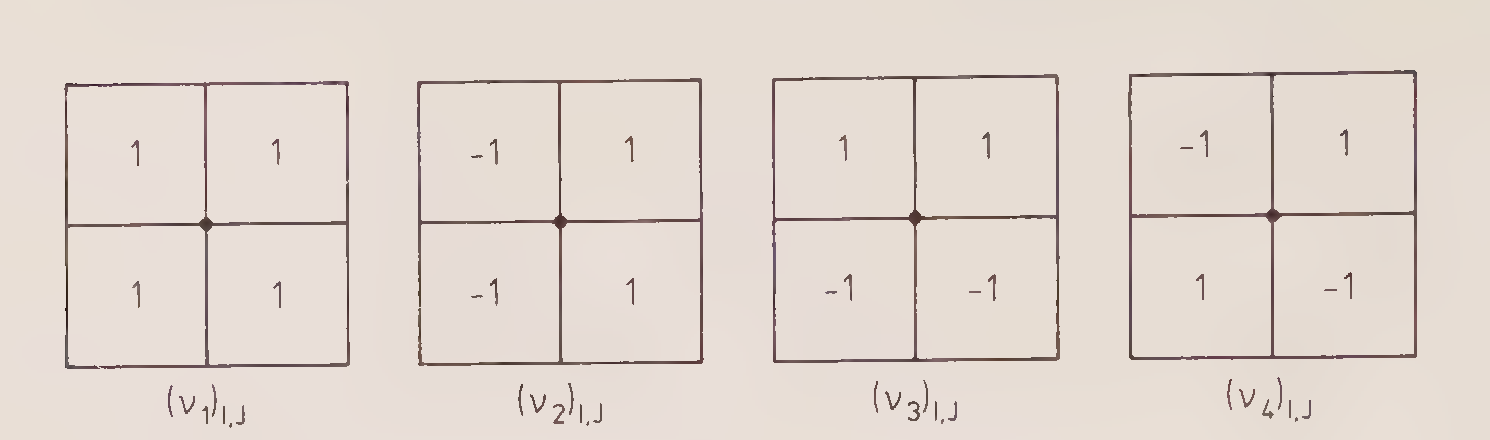
\includegraphics[width=.78\linewidth]{figures/chapter-02-figure-15.png}
\caption{宏单元上的四个分片常数基函数.}
\label{fig:primitive-macroelement-basis}
\end{figure}

并且
\begin{equation}\label{eq:primitive-macroelement-basis-orthogonality}
\int_{\Omega_{I,J}}(v_k)_{I,J}(v_l)_{I,J}\,dx=0
\qquad\text{当 }k\neq l.
\end{equation}
考虑 \eqref{eq:primitive-macroelement-basis-means}, 容易看出
\eqref{eq:primitive-q1-p0-spaces} 按如下方式定义 $M_h$:
\[
M_h=\left\{q=\sum_{I,J}\sum_{k=1}^{4}(\alpha_k)_{I,J}(v_k)_{I,J};
\ \sum_{I,J}(\alpha_1)_{I,J}=0\right\}.
\]
此外, 由于伪函数 $\mu$ 只能由``局部交替''函数 $v_4$ 产生,
由 \eqref{eq:primitive-macroelement-basis-orthogonality} 得
\[
[\operatorname{Ker}(B_h')]^\perp
=\left\{q=\sum_{I,J}\sum_{k=1}^{4}(\alpha_k)_{I,J}(v_k)_{I,J};
\ \sum_{I,J}(\alpha_1)_{I,J}=\sum_{I,J}(\alpha_4)_{I,J}=0\right\}.
\]
为简化记号, 令
\begin{equation}\label{eq:primitive-filtered-pressure-space}
\mathcal M_h=[\operatorname{Ker}(B_h')]^\perp.
\end{equation}

由于这里处理的是有限维空间, 空间对 $(X_h,\mathcal M_h)$ 满足 inf-sup 条件
\eqref{eq:primitive-discrete-inf-sup}. 可惜问题并未就此结束: 如下所示,
该条件关于 $h$ 并非一致地成立.

\setcounter{statement}{4}
\renewcommand{\theHstatement}{lemma.\thesection.\arabic{statement}}
\begin{Lemma}\label{lem:primitive-q1-p0-degenerate-inf-sup}
设 $\Omega$ 如上, 空间 $X_h$ 和 $\mathcal M_h$ 分别由
\eqref{eq:primitive-q1-p0-spaces} 和
\eqref{eq:primitive-filtered-pressure-space} 定义. 存在与 $h$ 无关的常数 $C>0$, 使
\begin{equation}\label{eq:primitive-q1-p0-h-inf-sup}
\sup_{\mathbf v\in X_h}
\left[\left(\int_\Omega q\operatorname{div}\mathbf v\,dx\right)
/|\mathbf v|_{1,\Omega}\right]
\geq Ch\|q\|_{0,\Omega}
\qquad\forall q\in\mathcal M_h.
\end{equation}
\end{Lemma}

\begin{Proof}
取 $\mathcal M_h$ 中任意函数 $q$, 引入离散半范数
\begin{equation}\label{eq:primitive-q1-p0-discrete-seminorm}
|q|_{1,h}=\left(\sum_{i,j}h^2
\{(\nabla_1q)_{i,j}^2+(\nabla_2q)_{i,j}^2\}\right)^{1/2},
\end{equation}
其中求和遍历 $\mathcal T_h$ 的所有内部节点 $(i,j)$. 由
\eqref{eq:primitive-q1-p0-summation-by-parts}, 定义 $X_h$ 中的函数
$\mathbf v=(u,v)$:
\[
u_{i,j}=-(\nabla_1q)_{i,j},
\qquad v_{i,j}=-(\nabla_2q)_{i,j}
\]

\MathBookSourcePage{179}
于 $\mathcal T_h$ 的所有内部节点 $(i,j)$ 上. 对此选择有
\[
\int_\Omega q\operatorname{div}\mathbf v\,dx=|q|_{1,h}^2,
\]
并由 Lemma~\ref{lem:appendix-local-inverse-inequality}, 直接计算得到
\[
|\mathbf v|_{1,\Omega}
\leq(C_1/h)\|\mathbf v\|_{0,\Omega}
\leq(C_2/h)|q|_{1,h}.
\]
因此
\[
\left(\int_\Omega q\operatorname{div}\mathbf v\,dx\right)
/|\mathbf v|_{1,\Omega}
\geq(h/C_2)|q|_{1,h},
\]
而若证明下面这个 Theorem~\ref{thm:h1-quotient-hilbert} 的类似式,
便得到 \eqref{eq:primitive-q1-p0-h-inf-sup}:
\begin{equation}\label{eq:primitive-q1-p0-discrete-poincare}
\|q\|_{0,\Omega}\leq C_3|q|_{1,h}
\qquad\forall q\in\mathcal M_h.
\end{equation}

下面证明 \eqref{eq:primitive-q1-p0-discrete-poincare}. 首先, 一个直接的构造性论证表明,
对于 $Q_h$ 中在两个单元 $\kappa_{i,j}$ 上为零的每个函数 $q$,
\eqref{eq:primitive-q1-p0-discrete-poincare} 均成立; 其中一个单元的 $i+j$ 为偶数,
另一个的 $i+j$ 为奇数. 当然, 常数 $C_3$ 与 $h,q$ 无关. 其次,
若 $q\in\mathcal M_h$, 容易找到 $\bar q\in\operatorname{Ker}(B_h')\oplus\mathbb R$,
使 $q-\bar q$ 具有上述性质. $q$ 与 $\bar q$ 的正交性于是给出
\[
\|q\|_{0,\Omega}^2
=\|q-\bar q\|_{0,\Omega}^2-\|\bar q\|_{0,\Omega}^2
\leq C_3^2|q-\bar q|_{1,h}^2=C_3^2|q|_{1,h}^2.
\]
\end{Proof}

很长时间里, 人们猜测 \eqref{eq:primitive-q1-p0-h-inf-sup} 无法改进;
但直到最近, Boland \& Nicolaides [12] 才用下面的反例证实了这一点.
粗略地说, 思路是寻找 $\mathcal M_h$ 中的函数 $q$, 使
\[
\left(\int_\Omega q\operatorname{div}\mathbf v\,dx\right)/|\mathbf v|_{1,\Omega}
\]
很小, 而 $\|q\|_{0,\Omega}$ 很大. 更准确地说, 令
\begin{equation}\label{eq:primitive-q1-p0-counterexample-pressure}
q=\sum_{I,J}\{I(v_4)_{I,J}\}.
\end{equation}
一方面, $I$ 遍历正负整数, 因而 $q$ 确实属于 $\mathcal M_h$.
另一方面, 直接计算表明
\[
\|q\|_{0,\Omega}^2
=4h^2(2n)\sum_I I^2
=4h(2n/3)(4n^2-1).
\]
因此
\begin{equation}\label{eq:primitive-q1-p0-counterexample-norm}
\|q\|_{0,\Omega}=[2/(\sqrt3h)](1-h^2)^{1/2}.
\end{equation}
接着计算 $\int_\Omega q\operatorname{div}\mathbf v\,dx$.
根据 \eqref{eq:primitive-q1-p0-discrete-gradients}, 有
\[
(\nabla_1q)_{i,j}=0\quad\forall i,j,
\qquad
(\nabla_2q)_{i,j}=
\begin{cases}
0,&i\text{ 为奇数},\\
(-1)^j(2/h),&i\text{ 为偶数}.
\end{cases}
\]
